\section{Evaluation}
\label{sec:evaluation}

Vermont and its modules have undergone extensive testing with respect to performance, interoperability and robustness.

\subsection{Performance}

Figure~\ref{fig_perf_sampler} shows the results obtained from benchmarking the sampler module on a dual-processor system\footnote{Dual 3.06GHz Intel Xeon, 2GB RAM, 1GBit NIC, Linux Kernel 2.6.13, libpcap-mmap 0.9.20060417}.
A specialized version~\cite{pcap-mmap} of the pcap library was used, which avoids multiple copying of captured data by mapping a user-space buffer into the kernel.
The traffic was generated using a packet generator set to fixed packet generation rates running on a separate machine. To ensure the desired packet rates, the UDP protocol was used.
%and the observed rate fluctuation averaged at 1.4\%.
Every two seconds, captured as well as dropped packets were accounted using the counters supplied by the pcap library. Multiple tests have proven the data sample shown in figure~\ref{fig_perf_sampler} to be Vermont's typical behavior over time.

Until a packet rate of 250,000 packets per second (for 128 byte packets), the capture rate is 100\%.
420,000 packets per second denotes the maximum packet generation rate and short-lived loss up to 45 percent can be observed; however, the loss is not of permanent nature and numerous measure points suggest the packet loss ratio being substantially smaller, averaging at 9.0 percent. At 300,000 packets per second the loss averages at 3.8 percent.
The diagram shows a certain fluctuation regarding the packet capture ratio. This stems from Vermont's asynchronous design utilizing buffered queues between subsystems. If the input queue suffers from congestion incoming packets will no longer be forwarded, but immediately dropped instead.
Capturing entire packets of 1500 bytes in size showed no loss at a maximum observed rate of 60,000 packets per second.

\begin{figure}
\begin{center}
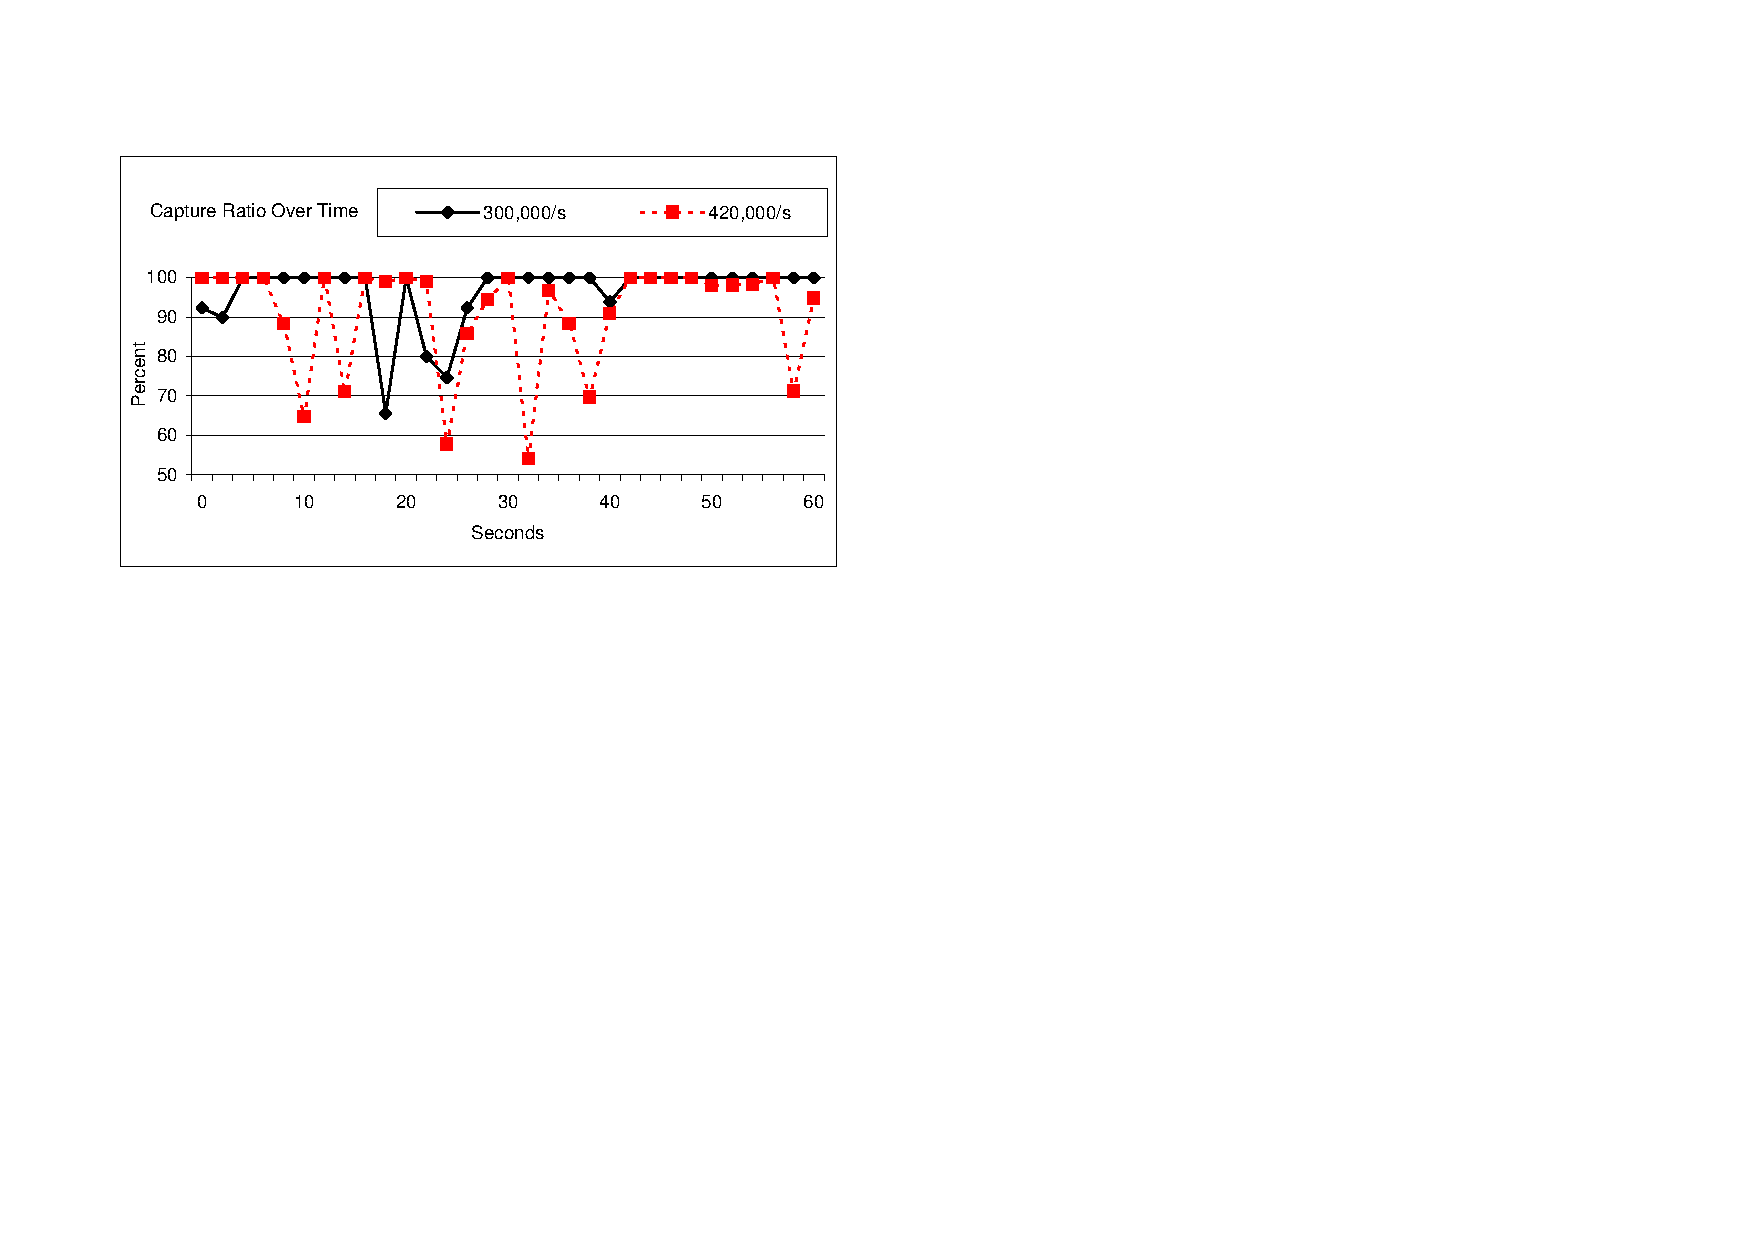
\includegraphics[scale=0.7]{gfx/sampler-perf3.pdf}
\caption{Capture ratio for packet rates of 300,000 and 420,000 packets per second}
\label{fig_perf_sampler}
\end{center}
\end{figure}

The concentrator module's performance was tested in a real-world scenario.
Vermont was configured to capture all packets at the access router of our university's network, perform flow accounting using the aggregation rule shown in figure~\ref{fig_rule}, and export the resulting records.
This rule creates standard IP-quintuple flow records with packet and byte counters.
During the tests, a maximum metering performance of 45,000 packets per second was achieved\footnote{Dual 2.0GHz Intel Xeon, 1GB RAM, 1GBit NIC, Linux Kernel 2.6.13, libpcap-mmap 1.0.20050129}. 
Repeating the test with different rule sets showed the maximum number of metered flows to be inversely proportional to the number of rules.
The big difference to the high packet rates measured with the sampler module alone shows that the flexible, rule-based aggregation scheme takes its toll.
We intend to improve this with an optimized flow accounting mechanism for standard IP-quintuple flows. 

\begin{figure}
\centering
\fbox{\begin{minipage}{7cm}
\scriptsize{\texttt {keep protocolIdentifier\\
keep sourcetransportport\\
keep sourceipv4address\\
keep destinationtransportport\\
keep destinationipv4address\\
aggregate inpacketdeltacount\\
aggregate inoctetdeltacount\\
aggregate flowcreationtime\\
aggregate flowendtime}
}
\end{minipage}}
\caption{Aggregation rule used by Concentrator module}
\label{fig_rule}
\end{figure}


\subsection{Interoperability and Robustness}

We participated in the IST MOME IPFIX Interoperability testing event~\cite{mome-interop} in July 2005 and tested Vermont's interoperability with several other IPFIX/PSAMP implementations. 
Vermont's collector and exporter successfully passed all applicable tests, including the handling of corrupt IPFIX data packets, and showed excellent robustness and compatibility.

